
% Paquetes
\documentclass[a4paper, 10pt, journal]{ieeeconf}
\overrideIEEEmargins
\usepackage[utf8]{inputenc}
\usepackage[T1]{fontenc}
\usepackage{fancyhdr}
\usepackage{lastpage}
\usepackage{graphicx}
\usepackage{amsmath}
\usepackage{amssymb} % Para símbolos matemáticos adicionales
\usepackage{adjustbox}
\graphicspath{{imágenes/}} 


% Configuración del encabezado y el pie de página
\pagestyle{fancy}
\fancyhf{}

% Encabezado
\fancyhead[L]{UNCuyo -- Ing. Mecatrónica \\ Mendoza - Argentina}
\fancyhead[C]{\textbf{311 -- AUTOMÁTICA Y MÁQUINAS ELÉCTRICAS \\ PROYECTO GLOBAL INTEGRADOR}}
\fancyhead[R]{Año: 2024 \\ Alumnos: Borquez y Escobar\\Fecha: 06/06/2024}

% Pie de página
\fancyfoot[C]{Página \thepage\ de \pageref{LastPage}} % Muestra "Página x de xx"

% Línea en la parte superior del encabezado
\renewcommand{\headrulewidth}{0.4pt}

% Línea en la parte inferior del pie de página
\renewcommand{\footrulewidth}{0.4pt}

% Título
\title{\LARGE \bf
Proyecto Global Integrador: Control de Accionamiento de CA con
Motor Sincrónico de Imanes Permanentes
}

\author{Borquez Juan y Escobar Matías}

\begin{document}

\maketitle
\thispagestyle{empty}
\pagestyle{fancy}

% RESUMEN
\begin{abstract}
\end{abstract}

% INTRODUCCIÓN
\section{INTRODUCCIÓN}
Modelado, simulación, diseño y análisis de desempeño de un Sistema de Control Automático de Posición y Movimiento para un Accionamiento electromecánico de 4 cuadrantes, compuesto por: máquina eléctrica de corriente alterna (CA) trifásica sincrónica con excitación por imanes permanentes (PMSM), alimentada por inversor trifásico desde fuente de corriente continua (CC); reductor de velocidad de engranajes planetarios de salida hacia la carga mecánica; realimentación con 1 sensor de posición en el eje del motor, más 3 sensores de corriente instantánea de fases en la salida del inversor trifásico al estator de la máquina (PMSM) y 1 sensor de temperatura del bobinado de estator.


% DESARROLLO - PRESENTACIÓN DEL PROBLEMA
\section{PRESENTACIÓN DEL PROBLEMA}
\subsection{\textbf{Carga Mecánica}}
Aplicación simplificada de referencia (adaptado de \cite{c1}): control de movimiento de 1 eje (descentralizado) para articulación de brazo manipulador robótico elemental de un grado de libertad (1 g.d.l.) rotacional de eje horizontal sometido a la acción de la aceleración de gravedad (péndulo rígido actuado), con eje de rotación fijo a base en sistema de referencia inercial (Fig. \ref{brazo}); con parámetros equivalentes variables según sea la carga útil transportada en el extremo (ver Ec. \ref{subsistema mecánico referido a eje de salida}).

\begin{figure}[thpb]
    \centering
    \begin{adjustbox}{max width=\columnwidth}
        \framebox{\parbox{\columnwidth}{
            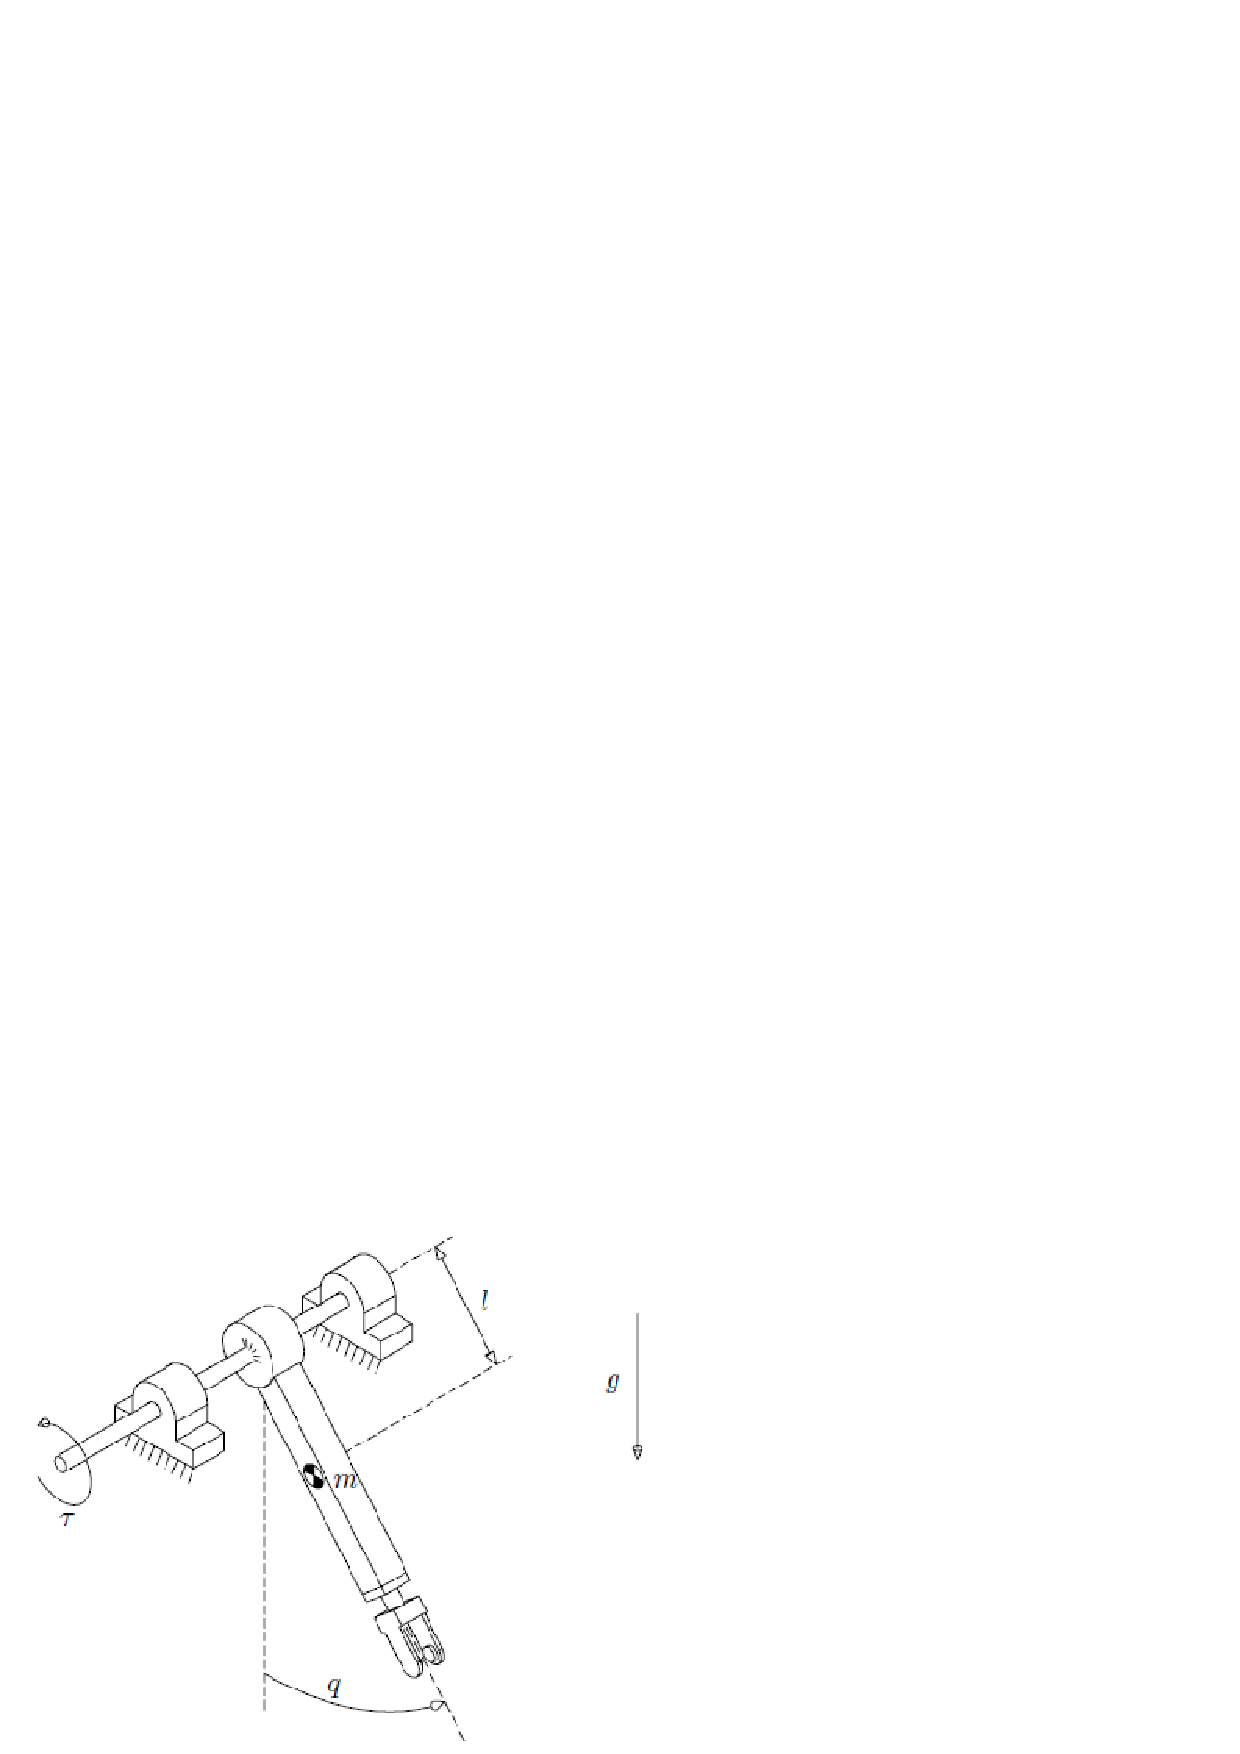
\includegraphics[width=\columnwidth]{1-Brazo.PNG}
        }}
    \end{adjustbox}
    \caption{Robot manipulador elemental de 1 g.d.l. en plano vertical (péndulo rígido actuado) \cite{c2}.}
    \label{brazo}
\end{figure}
\bigskip


\subsubsection{\textbf{Modelo}} simplificado equivalente (No Lineal con parámetros variables), referido al eje de salida del tren de transmisión: coordenada articular de eje de la articulación $q(t) \equiv \theta_l(t)$, referida a la vertical hacia abajo, positiva en sentido antihorario; torque impulsor $\tau(t) \equiv T_q(t)$.

\begin{equation}
    J_l \frac{d\omega_l(t)}{dt} = T_q(t) - b_l \omega_l(t) - T_l(t)
    \label{subsistema mecánico referido a eje de salida}
\end{equation}
\begin{equation}
    T_l(t) = k_l \sin(\theta_l(t)) + T_d(t)
    \label{torque de carga}
\end{equation}
\begin{equation}
    \frac{d\theta_l(t)}{dt} \equiv \omega_l(t) \Leftrightarrow \theta_l(t) = \int_{0}^{t} \omega_l(\zeta) \, d\zeta + \theta_l(0))
    \label{velocidad y posición de la carga}
\end{equation}



\subsubsection{\textbf{Parámetros Equivalentes Variables}}
\begin{itemize}
    \item Coeficiente de fricción viscosa en articulación:
    \[
    b_l \approx (0.1 \pm 0.03) \, \text{N.m rad/s} \text{(incertidumbre)}
    \]
    \item Aceleración de gravedad:
    \[
    g = 9.80665 \, \text{m/s}^2
    \]
    \item Masa del brazo manipulador:
    \[m = 1.0 \, \text{kg}
    \]
    \item Longitud e Inercia equivalente (resepcto al centro de masa):
    \begin{align*}
    l_{\text{cm}} &= 0.25 \, \text{m} \\
    J_{\text{cm}} &= 0.0208 \, \text{kg}\cdot\text{m}^2
    \end{align*}
    \item Longitud total (extremo):
    \[
    l_l = 0.50 \, \text{m}
    \]
    \item Masa de carga útil en el extremo (variable):
    \[
    m_l = [0 \, \ldots \, 1.5] \, \text{kg}
    \]
    \item Momento de inercia total (respecto al eje de rotación): 
    \[
    J_l = (m \cdot l_{cm}^2 + J_{cm}) + m_l \cdot l_l^2 = 0.0833 + [0 \, \ldots \, 0.375] \, \text{kg.m}^2
    \]
    \item Coeficiente de torque recuperador gravitacional: 
    \[
    k_l = m \cdot g \cdot l_{cm} + m_l \cdot g \cdot l_l = 2.452 + [0 \, \ldots \, 7.355] \, \text{N.m}
    \]
\end{itemize}



\subsubsection{\textbf{Especificaciones de Operación}}
\begin{itemize}
    \item Torque de perturbación externo:
    \[T_d(t) \approx (0 \pm 5.0) \, \text{N.m}
    \]
\end{itemize}



\subsection{\textbf{Caja Reductora}}
Caja reductora reversible con sistema de engranajes planetarios, asumiendo acoplamiento rígido (sin elasticidad torsional y sin juego, holgura o ``backlash''); momento de inercia equivalente y pérdidas de energía por fricción interna, reflejados al eje de entrada y considerados junto con el motor
\bigskip



\subsubsection{\textbf{Modelo equivalente (rígido)}}
\begin{equation}
    \omega_l(t) = 1/r \cdot \omega_m(t)
    \label{relación de velocidad en caja}
\end{equation}
\begin{equation}
    T_q(t) = r \cdot T_{dm}(t)
    \label{relación de torque en caja}
\end{equation}



\subsubsection{\textbf{Parámetros}}
\begin{itemize}
    \item Relación de reducción total:
    \[
    r = 120.0 : 1
    \]
\end{itemize}



\subsubsection{\textbf{Especificaciones de operación}}:
\begin{itemize}
    \item Velocidad nominal (salida):
    \[
    n_{lnom} = 60\ rpm \ (\omega_{lnom} = 6.28 \ rad/s)
    \]
    \item Torque nominal (salida):
    \[
    T_{qnom} = 17.0 \, N.m \ \text{(régimen continuo o rms)}
    \]
    \item Torque pico (salida):
    \[
    T_{qmax} = 45.0 \, N.m \ \text{(corta duración, aceleración)}
    \]
\end{itemize}



\subsection{\textbf{Máquina Eléctrica PMSM}}
Máquina eléctrica de CA trifásica sincrónica con excitación por imanes permanentes (PMSM) y estator conectado en estrella (simétrico y equilibrado) accesible en bornes de fases $abc$, con centro de estrella (punto “neutro”) flotante (no accesible).



\subsubsection{\textbf{Subsistema mecánico}}
Rotor referido a Estator estacionario (fijo a sistema inercial de referencia).

\begin{equation}
    J_m \frac{d\omega_m(t)}{dt} = T_m(t) - b_m \omega_m(t) - T_{dm}(t)
    \label{subsistema mecánico máquina eléctrica}
\end{equation}
\begin{equation}
    \frac{d\theta_m(t)}{dt} \equiv \omega_m(t) \Leftrightarrow \theta_m(t) = \int_{0}^{t} \omega_m(\tau) d\tau + \theta_m(0)
    \label{posición y velocidad motor}
\end{equation}



\subsubsection{\textbf{Subsistema electromagnético}} Modelo idealizado equivalente en coordenadas eléctricas de entrehierro $qd0^{r}$ fijas a rotor, aplicando Transformación de Park a circuito estator estacionario (\cite{c3}).
\begin{itemize}
    \item Coordenadas eléctricas de entrehierro $qd0^{r}$ (marco de referencia de rotor $\neq$ “sincrónico”):
    \begin{equation}
        \frac{d\theta_r(t)}{dt} \equiv \omega_r(t) \Leftrightarrow \theta_r(t) = \int_{0}^{t} \omega_r(\tau) d\tau + \theta_r(0)
        \label{Relación coordenadas eléctricas y mecánicas}
    \end{equation}
    \begin{equation}
        \theta_r(t) \equiv P_p \theta_m(t) \therefore  \omega_r(t) = P_p \omega_m(t)
        \label{posicion y velocidad rotor}
    \end{equation}
    \item Torque electromagnético:
    \begin{flalign}
        \resizebox{0.88125\linewidth}{!}{
            $T_m(t) = \frac{3}{2} P_p [\lambda'^r_{m} i^r_{qs}(t) + (L_d - L_q) i^r_{ds}(t) i^r_{qs}(t)$]}&
        \label{torque electromagnético}
    \end{flalign}
    \item Balance de tensiones eléctricas equivalentes de estator (referido a coordenadas $qd0^{r}$):
    \begin{flalign}
        \resizebox{0.88125\linewidth}{!}{
            $v^r_{qs}(t) = R_s(t) i^r_{qs}(t) + L_q \frac{di^r_{qs}(t)}{dt} + [\lambda'^r_{m} + L_d i^r_{ds}(t)] \omega_r(t)$} &
        \label{balance de tensiones q}
    \end{flalign}
    \begin{flalign}
        \resizebox{0.88125\linewidth}{!}{
            $v^r_{ds}(t) = R_s(t) i^r_{ds}(t) + L_d \frac{di^r_{ds}(t)}{dt} - L_q i^r_{qs}(t) \omega_r(t)$} &
        \label{balance de tensiones d}
    \end{flalign}
    \begin{equation}
        v_{0s}(t) = R_s(t) i_{0s}(t) + L_{ls} \frac{di_{0s}(t)}{dt}
        \label{balance de tensiones 0}
    \end{equation}
    \begin{equation}
        R_s(t) = R_{sREF} \left(1 + \alpha_{Cu} (T_s^{\circ}(t) - T_{sREF}^{\circ})\right)
        \label{Rs}
    \end{equation}
\end{itemize}

\subsubsection{\textbf{Subsistema Térmico}} Modelo simplificado equivalente de primer orden, considerando sólo pérdidas
eléctricas resistivas por efecto Joule en bobinado de estator, despreciando pérdidas magnéticas
en el núcleo; transferencia de calor por conducción y convección natural, sin ventilación forzada:
\begin{itemize}
    \item Potencia de pérdidas calóricas:
    \begin{align}
        P_{s\ perd}(t) &= R_s(t) \left(i_{as}^2(t) + i_{bs}^2(t) + i_{cs}^2(t)\right) \nonumber \\
        &= \frac{3}{2} R_s(t) \left(i_{qs}^2(t) + i_{ds}^2(t) + 2 i_{0s}^2(t)\right)
        \label{potencia de perdidas}
    \end{align}
    \item Balance térmico de estator:
    \begin{flalign}
        \resizebox{0.88125\linewidth}{!}{
            $P_{s\ perd}(t) = C_{ts} \frac{dT_s^{\circ}(t)}{dt} + \frac{1}{R_{ts-amb}} \left(T_s^{\circ}(t) - T_{amb}^{\circ}(t)\right)$}
        \label{balance térmico estator}
    \end{flalign}
\end{itemize}

\subsubsection{\textbf{Parámetros}} Valores nominales medidos, tolerancia error $\pm$ 1\%; salvo aclaración específica:
\begin{itemize}
    \item Momento de inercia (motor y caja):
    \[J_m \approx 1.4 \times 10^{-5} \, \text{kg} \cdot \text{m}^2\]
    \item Coef. de fricción viscosa (motor y caja):
    \[b_m \approx 1.5 \times 10^{-5} \, \text{N} \cdot \text{m} \cdot \text{s}^{-1} \cdot \text{rad}^{-1}\]
    \item Pares de Polos magnéticos: 
    \[P_p = 3\]
    \item Flujo magnético equivalente de imanes concatenado por espiras del bobinado de estator:
    \[\lambda_m'^{r} \approx 0.016 \, \text{Wb} \\-\\ \left(\frac{V}{rad/s}\right)\]
    \item Inductancia de estator (eje en cuadratura):
    \[L_q \approx 5.8 \, \text{mH}\]
    \item Inductancia de estator (eje directo):
    \[L_d \approx 6.6 \, \text{mH}\]
    \item Inductancia de dispersión de estator:
    \[L_{ls} \approx 0.8 \, \text{mH}\]
    \item Resistencia de estator, por fase (Ec. 3.9):
    \[R_s \approx 1.02 \, \Omega \ (@40 ^\circ C) \rightarrow 1.32 \Omega \ (@115 ^\circ C)\]
    \item Coef. aumento de $R_s$ con $T_s^\circ(t)$ (\ref{Rs}): \[\alpha_C = 3.9 \times 10^{-3} \, ^{\circ}\text{C}^{-1}\]
    \item Capacitancia térmica de estator:
    \[C_{ts} \approx 0.818 \, \text{W} \cdot ^{\circ}\text{C}^{-1} \cdot \text{s}^{-1}\]
    \item Resistencia térmica estator-ambiente:
    \[R_{ts-\text{amb}} \approx 146.7 \, ^{\circ}\text{C} \cdot \text{W}^{-1}\]
\end{itemize}
Nota: Constante de tiempo térmica:
\[\tau_{ts-\text{amb}} = R_{ts-\text{amb}} \cdot C_{ts} \approx 120 \, \text{s}\]

































\section{DESARROLLO DE TAREAS}


\subsection{\textbf{Modelado, Análisis y Simulación dinámica del SISTEMA FÍSICO a “Lazo
Abierto” (Sin Controlador externo de Movimiento)}}



\subsubsection{\textbf{Modelo sub-sistema mecánico completo}}
Multiplicando por $r$ ambos miembros de la ecuación (\ref{subsistema mecánico máquina eléctrica}), sumando miembro a miembro con la ecuación (\ref{subsistema mecánico referido a eje de salida}) y tomando en cuenta $T_q(t)$ según la ecuación (\ref{relación de torque en caja}) obtenemos:

\begin{flalign*}
    \resizebox{0.95\linewidth}{!}{
        $
        J_{l}\,\frac{d\omega _{l}\left(t\right)}{dt} +J_{m}\,r\,\frac{d\omega _{m}\left(t\right)}{dt} =r\,T_{m}\left(t\right)-T_{l}\left(t\right)-b_{l}\,\omega _{l}\left(t\right)-b_{m}\,r\,\omega _{m}\left(t\right)
        $}
\end{flalign*}
Reemplazando en la anterior $\omega_{l}(t)$ según la ecuación (\ref{relación de velocidad en caja}), agrupando términos y diviendo entre $r$ a ambos miembros, obtenemos:
\begin{flalign}
    \resizebox{0.89125\linewidth}{!}{
        $
        \left(J_{m}+\frac{J_{l}}{r^2}\right)\,\frac{d \omega _{m}\left(t\right)}{dt}=T_{m}\left(t\right)-\left(b_{m}+\frac{b_{l}}{r^2}\right)\,\omega _{m}\left(t\right)-\frac{T_{l}\left(t\right)}{r}
        $}
    \label{subsistema mecánico con parametros desarrollados}
\end{flalign}
Definimos ahora la inercia equivalente y el amoriguamiento equivalente respectivamente como:
\begin{equation}
   J_{eq}= \left(J_{m}+\frac{J_{l}}{r^2}\right)
   \label{inercia equivalente}
\end{equation}
\begin{equation}
    b_{eq}=\left(b_{m}+\frac{b_{l}}{r^2}\right)
    \label{amortiguamiento equivalente}
\end{equation}
Reemplazando (\ref{inercia equivalente}) y (\ref{amortiguamiento equivalente}) en (\ref{subsistema mecánico con parametros desarrollados}) obtenemos el modelo matemático equivalente del sub-sistema mecánico completo con parámetros equivalentes referido aleje del motor (veasé diagrama de bloques de la fig. \ref{diagrama de bloques sub-sistema mecánico completo}):
\begin{flalign}
    \resizebox{0.89125\linewidth}{!}{
        $
        J_{eq}\,\frac{d \omega _{m}\left(t\right)}{dt}=T_{m}\left(t\right)-b_{eq}\, \omega _{m}\left(t\right)-\frac{T_{l}\left(t\right)}{r}
        $}
        \label{subsistema mecánico con parametros equivalentes}
\end{flalign}
\begin{figure}[thpb]
    \centering
    \begin{adjustbox}{max width=\columnwidth}
        \framebox{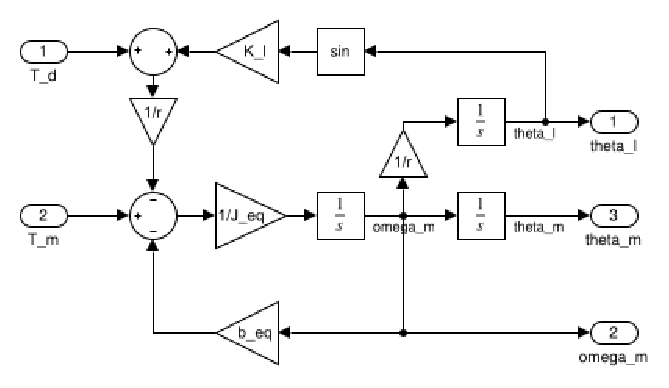
\includegraphics{2-Subsistema_Mecánico_Completo.eps}}
    \end{adjustbox}
    \caption{Diagrama de bloques del sub-sistema mecánico completo.}
    \label{diagrama de bloques sub-sistema mecánico completo}
\end{figure}

El modelo resultante tiene un solo grado de libertad, tal como sucede en el modelo de la carga y del subsistema mecánico de la máquina eléctrica sin la transmisión. Esto se debe a la rigidez y la ausencia de "backlash" en la reducción, permitiendo un "acoplamiento directo" de la carga al eje de la máquina. Dicho de otra manera, la transmisión no incorpora dinámica al subsistema mecánico completo.



\subsubsection{\textbf{Modelo dinámico del sistema físico completo}}
\paragraph{\textbf{Modelo Global No Lineal}}
En la Figura \ref{diagrama de bloques del sistema físico} se muestra
el diagrama de bloques del sistema físico completo, el cual está compuesto por varios subsistemas. En las Figuras \ref{subsistema térmico}, \ref{diagrama de bloques sub-sistema mecánico completo},
\ref{subsistema electromagnético} se muestran los diagramas de bloques de los subsistemas térmico, mecánico y electromagnético respectivamente. A su vez, los componentes del sub-sistema electromagnético se detallan
en las figuras \ref{diagrama de bloques I_qs}, \ref{diagrama de bloques I_ds}, \ref{diagrama de bloques I_0s}, para las corrientes ($i_{qs}$, $i_{ds}$, $i_{0s}$ respectivamente) y \ref{diagrama de bloques T_m} para el torque motor.
En las figuras \ref{transformación de park} y \ref{transformación de park inversa} se detallan las transformaciones de Park directa e inversa respecticamente.

\begin{multicols}{2}
    \begin{align*}
        \frac{d}{dt} \begin{bmatrix} \theta_m \\ \omega_m \\ i^r_{qs} \\ i^r_{ds} \\ i_{0s} \\ T_s \end{bmatrix} &= \begin{bmatrix} \omega_m \\ \frac{3}{2} \frac{P_p i^r_{qs}(t)}{J_{eq}} \left[ \lambda'^r_{m} + (L_d - L_q) i^r_{ds}(t) \right] - \frac{b_{eq}}{J_{eq}} \omega_m(t) - \frac{T_l(t)}{J_{eq}r} \\ \frac{1}{L_q} \left( v^r_{qs}(t) - R_s(t) i^r_{qs} - [\lambda'^r_m + L_d i^r_{ds}] \omega_r(t) \right) \\ \frac{1}{L_d} \left( v^r_{ds}(t) - R_s(t) i^r_{ds} + L_q i^r_{qs} \omega_r(t) \right) \\ \frac{1}{L_{ls}} \left( v_{0s}(t) - R_s(t) i_{0s} \right) \\ \frac{3}{2} \frac{R_s(t)}{C_{ts}} \left( i_{qs}^2(t) + i_{ds}^2(t) + 2 i_{0s}^2(t) \right) - \frac{1}{C_{ts}R_{ts-amb}} (T_s - T_{amb}) \end{bmatrix}
    \end{align*}
\end{multicols}


\begin{figure}[thpb]
    \centering
    \begin{adjustbox}{max width=\columnwidth}
        \framebox{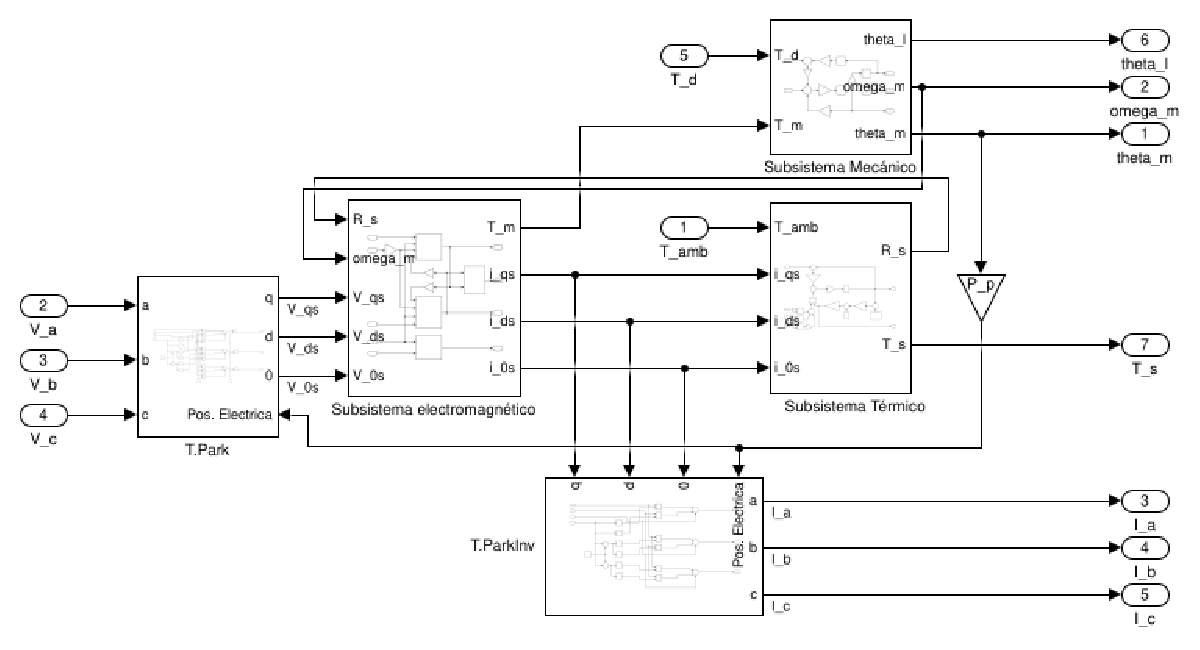
\includegraphics{9-Sistema_Físico_Completo.eps}}
    \end{adjustbox}
    \caption{Diagrama de bloques del sistema físico completo.}
    \label{diagrama de bloques del sistema físico}
\end{figure}
\begin{figure}[thpb]
    \centering
    \begin{adjustbox}{max width=\columnwidth}
        \framebox{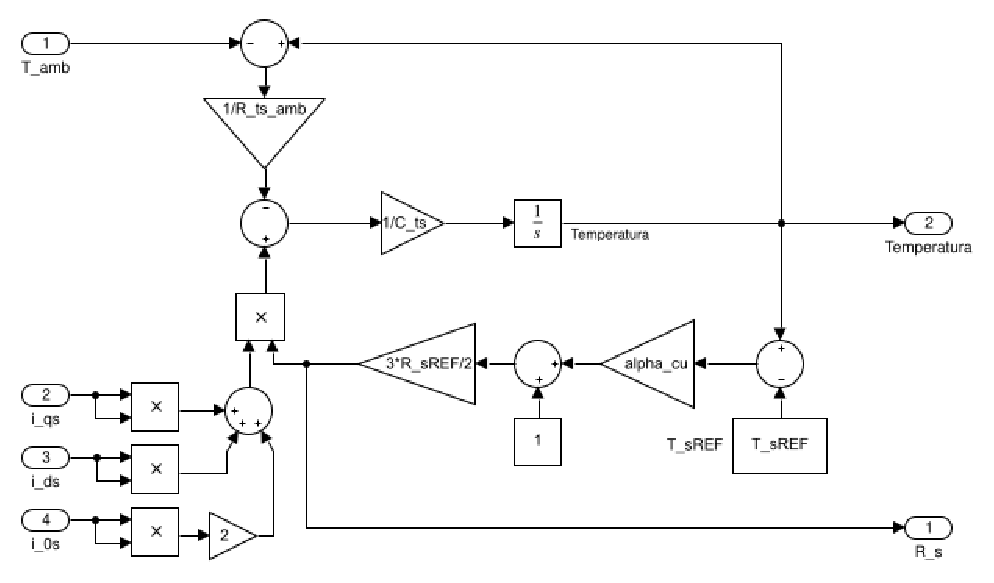
\includegraphics{3-Subsistema_Térmico.eps}}
    \end{adjustbox}
    \caption{Diagrama de bloques del sub-sistema térmico}
    \label{subsistema térmico}
\end{figure}
\begin{figure}[thpb]
    \centering
    \begin{adjustbox}{max width=\columnwidth}
        \framebox{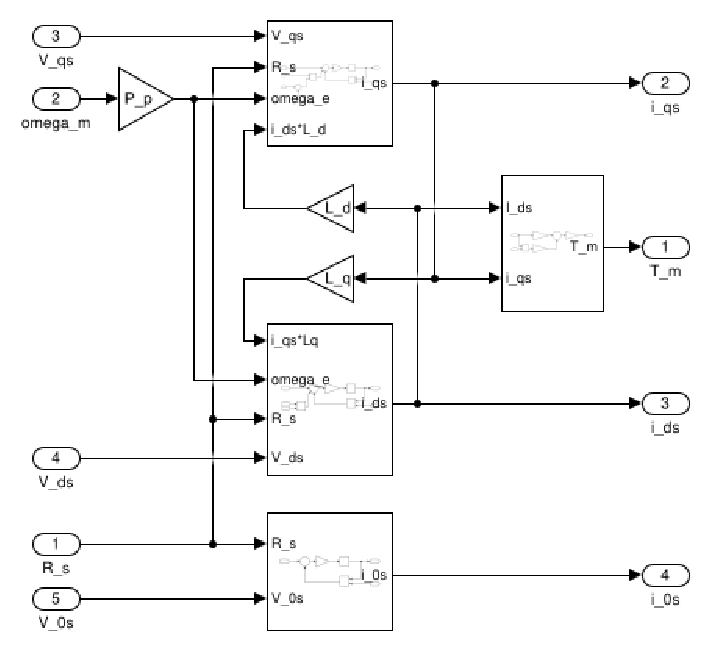
\includegraphics{8-Subsistema_Electromagnético.eps}}
    \end{adjustbox}
    \caption{Diagrama de bloques del sub-sistema electromagnético}
    \label{subsistema electromagnético}
\end{figure}
\begin{figure}[thpb]
    \centering
    \begin{adjustbox}{max width=\columnwidth}
        \framebox{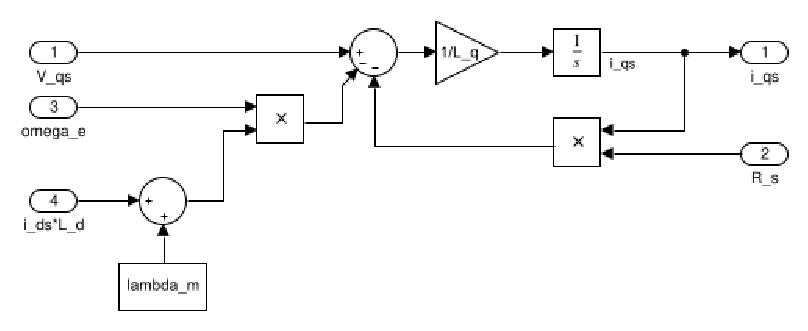
\includegraphics{4-I_qs.eps}}
    \end{adjustbox}
    \caption{Diagrama de bloques $I_{qs}$}
    \label{diagrama de bloques I_qs}
\end{figure}
\begin{figure}[thpb]
    \centering
    \begin{adjustbox}{max width=\columnwidth}
        \framebox{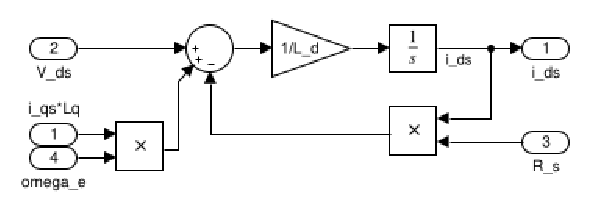
\includegraphics{5-I_ds.eps}}
    \end{adjustbox}
    \caption{Diagrama de bloques $I_{ds}$}
    \label{diagrama de bloques I_ds}
\end{figure}
\begin{figure}[thpb]
    \centering
    \begin{adjustbox}{max width=\columnwidth}
        \framebox{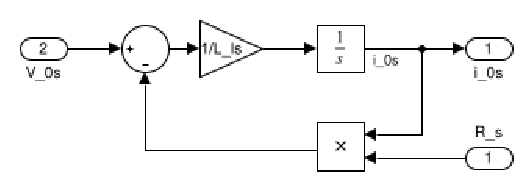
\includegraphics{6-I_0s.eps}}
    \end{adjustbox}
    \caption{Diagrama de bloques $I_{0s}$}
    \label{diagrama de bloques I_0s}
\end{figure}
\begin{figure}[thpb]
    \centering
    \begin{adjustbox}{max width=\columnwidth}
        \framebox{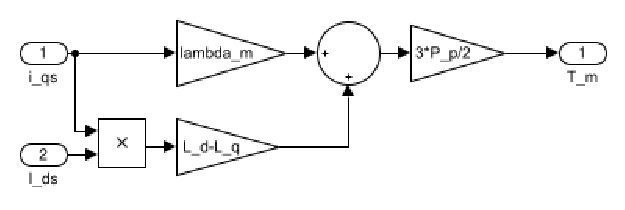
\includegraphics{7-T_m.eps}}
    \end{adjustbox}
    \caption{Diagrama de bloques $T_m$}
    \label{diagrama de bloques T_m}
\end{figure}
\begin{figure}[thpb]
    \centering
    \begin{adjustbox}{max width=\columnwidth}
        \framebox{\includegraphics{10-Transformación_de_Park.eps}}
    \end{adjustbox}
    \caption{Transformación de Park Directa}
    \label{transformación de park}
\end{figure}
\begin{figure}[thpb]
    \centering
    \begin{adjustbox}{max width=\columnwidth}
        \framebox{\includegraphics{11-Transformación_de_Park_Inversa.eps}}
    \end{adjustbox}
    \caption{Transformación de Park Inversa}
    \label{transformación de park inversa}
\end{figure}




























\section{ANÁLISIS DE RESULTADOS}


\subsection{Heading 1, etc}


\subsection{Figures and Tables}

Positioning Figures and Tables: Place figures and tables at the top and bottom of columns. Avoid placing them in the middle of columns. Large figures and tables may span across both columns. Figure captions should be below the figures; table heads should appear above the tables. Insert figures and tables after they are cited in the text. Use the abbreviation ``Fig. 1'', even at the beginning of a sentence.

\begin{table}[h]
\caption{An Example of a Table}
\label{table_example}
\begin{center}
\begin{tabular}{|c||c|}
\hline
One & Two\\
\hline
Three & Four\\
\hline
\end{tabular}
\end{center}
\end{table}


   \begin{figure}[thpb]
      \centering
      \framebox{\parbox{3in}{We suggest that you use a text box to insert a graphic (which is ideally a 300 dpi TIFF or EPS file, with all fonts embedded) because, in an document, this method is somewhat more stable than directly inserting a picture.
}}
      %\includegraphics[scale=1.0]{figurefile}
      \caption{Inductance of oscillation winding on amorphous
       magnetic core versus DC bias magnetic field}
      \label{figurelabel}
   \end{figure}

\section{CONCLUSIONES}


\addtolength{\textheight}{-12cm}   % This command serves to balance the column lengths
                                  % on the last page of the document manually. It shortens
                                  % the textheight of the last page by a suitable amount.
                                  % This command does not take effect until the next page
                                  % so it should come on the page before the last. Make
                                  % sure that you do not shorten the textheight too much.

%%%%%%%%%%%%%%%%%%%%%%%%%%%%%%%%%%%%%%%%%%%%%%%%%%%%%%%%%%%%%%%%%%%%%%%%%%%%%%%%



%%%%%%%%%%%%%%%%%%%%%%%%%%%%%%%%%%%%%%%%%%%%%%%%%%%%%%%%%%%%%%%%%%%%%%%%%%%%%%%%



%%%%%%%%%%%%%%%%%%%%%%%%%%%%%%%%%%%%%%%%%%%%%%%%%%%%%%%%%%%%%%%%%%%%%%%%%%%%%%%%
\section*{APENDICE}

Appendixes should appear before the acknowledgment.

\begin{thebibliography}{99}

\bibitem{c1} G. O. Young, ``Synthetic structure of industrial plastics (Book style with paper title and editor),'' 	in Plastics, 2nd ed. vol. 3, J. Peters, Ed.  New York: McGraw-Hill, 1964, pp. 15--64.
\bibitem{c2} R. Kelly et al, Control of Robot Manipulators in Joint Space. Springer, 2005. (Example and Figure 2.2).
\bibitem{c3} P. Krause et al, Analysis of Electric Machinery and Drive Systems, 3rd Ed.. IEEE-Wiley, 2013.
\bibitem{c4} B. Smith, ``An approach to graphs of linear forms (Unpublished work style),'' unpublished.
\bibitem{c5} E. H. Miller, ``A note on reflector arrays (Periodical styleÑAccepted for publication),'' IEEE Trans. Antennas Propagat., to be publised.
\bibitem{c6} J. Wang, ``Fundamentals of erbium-doped fiber amplifiers arrays (Periodical styleÑSubmitted for publication),'' IEEE J. Quantum Electron., submitted for publication.

\end{thebibliography}

Matrices Modelo linealizado
\begin{equation*}\label{eq:matriz_A}
\resizebox{\textwidth}{!}{
$A = \left(\begin{array}{cccccc} 
0 & 1 & 0 & 0 & 0 & 0\\ 
-\frac{K_{l}\,\cos\left(\frac{\theta _{m}}{r}\right)}{J_{\mathrm{eq}}\,r^2} & -\frac{b_{\mathrm{eq}}}{J_{\mathrm{eq}}} & \frac{3\,\mathrm{Pp}\,\left(\lambda _{m}+i_{\mathrm{ds}}\,\left(L_{d}-L_{q}\right)\right)}{2\,J_{\mathrm{eq}}} & \frac{3\,\mathrm{Pp}\,i_{\mathrm{qs}}\,\left(L_{d}-L_{q}\right)}{2\,J_{\mathrm{eq}}} & 0 & 0\\ 
0 & -\frac{3\,\mathrm{Pp}\,i_{\mathrm{ds}}\,\left(L_{d}+\lambda _{m}\right)}{2\,L_{q}} & -\frac{R_{\mathrm{sref}}\,\left(\alpha _{\mathrm{cu}}\,\left(T_{s}-T_{\mathrm{sref}}\right)+1\right)}{L_{q}} & -\frac{L_{d}\,\mathrm{Pp}\,\omega _{m}}{L_{q}} & 0 & -\frac{R_{\mathrm{sref}}\,\alpha _{\mathrm{cu}}\,i_{\mathrm{qs}}}{L_{q}}\\ 
0 & \frac{L_{q}\,\mathrm{Pp}\,i_{\mathrm{qs}}}{L_{d}} & \frac{L_{q}\,\mathrm{Pp}\,\omega _{m}}{L_{d}} & -\frac{R_{\mathrm{sref}}\,\left(\alpha _{\mathrm{cu}}\,\left(T_{s}-T_{\mathrm{sref}}\right)+1\right)}{L_{d}} & 0 & -\frac{R_{\mathrm{sref}}\,\alpha _{\mathrm{cu}}\,i_{\mathrm{ds}}}{L_{d}}\\ 
0 & 0 & 0 & 0 & -\frac{R_{\mathrm{sref}}\,\left(\alpha _{\mathrm{cu}}\,\left(T_{s}-T_{\mathrm{sref}}\right)+1\right)}{L_{\mathrm{ls}}} & -\frac{R_{\mathrm{sref}}\,\alpha _{\mathrm{cu}}\,i_{\mathrm{os}}}{L_{\mathrm{ls}}}\\ 
0 & 0 & \frac{3\,R_{\mathrm{sref}}\,i_{\mathrm{qs}}\,\left(\alpha _{\mathrm{cu}}\,\left(T_{s}-T_{\mathrm{sref}}\right)+1\right)}{C_{\mathrm{ts}}} & \frac{3\,R_{\mathrm{sref}}\,i_{\mathrm{ds}}\,\left(\alpha _{\mathrm{cu}}\,\left(T_{s}-T_{\mathrm{sref}}\right)+1\right)}{C_{\mathrm{ts}}} & \frac{6\,R_{\mathrm{sref}}\,i_{\mathrm{os}}\,\left(\alpha _{\mathrm{cu}}\,\left(T_{s}-T_{\mathrm{sref}}\right)+1\right)}{C_{\mathrm{ts}}} & \frac{R_{\mathrm{sref}}\,\alpha _{\mathrm{cu}}\,\left(3\,{i_{\mathrm{ds}}}^2+6\,{i_{\mathrm{os}}}^2+3\,{i_{\mathrm{qs}}}^2\right)}{2\,C_{\mathrm{ts}}}-\frac{1}{C_{\mathrm{ts}}\,R_{\mathrm{ts},\mathrm{amb}}} 
\end{array}\right)$
}
\end{equation*}


\end{document}